\newpage

\section{Register Allocation}

In this section\cite{REGISTER78:online} we discuss register allocation, which is one of the last steps
in a compiler before code emission. Its task is to map the potentially unbounded numbers of variables or “temps” in pseudo-assembly to the actually available registers on the target machine. If not enough registers are
available, some values must be saved to and restored from the stack, which
is much less efficient than operating directly on registers. Register allocation is therefore of crucial importance in a compiler and has been the subject of much research. Register allocation is also covered thorougly in the
textbook, but the algorithms described there are complicated and difficult to implement. We present here a simpler algorithm
for register allocation based on chordal graph coloring due to Hack \cite{hack2006register}
and Pereira and Palsberg [PP05]. Pereira and Palsberg have demonstrated
that this algorithm performs well on typical programs even when the interference graph is not chordal. The fact that we target the x86-64 family
of processors also helps, because it has 16 general registers so register allocation is less important than for the x86 with only 8 registers (ignoring
floating-point and other special purpose registers).
Most of material below is based on Pereira and Palsberg \cite{pereira2005register}, where
further background, references, details, empirical evaluation, and examples can be found.




\subsection{Graph Coloring}


Register allocation via graph coloring, like linear-scan register allocation, considers allocating registers to variables across a whole procedure. However, it uses live ranges instead of live intervals. This addresses the problem mentioned above with linear scan allocation, namely that if there are "holes" in a variable's live interval, then it can be wasteful to tie up a register for the entire live interval (as illustrated below).


\begin{figure}[H]
	\centering
	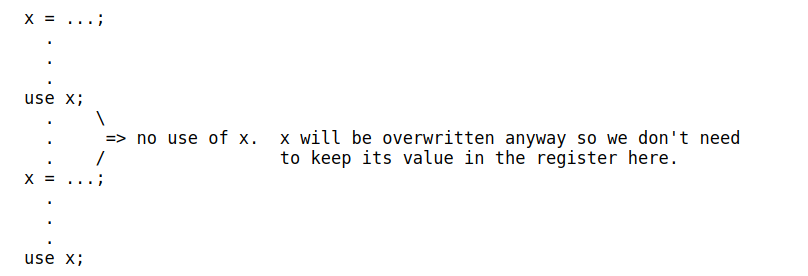
\includegraphics[width=0.6\textwidth]{p163.png}
	\caption{Motivation for graph coloring}
	\label{fig:p163}
\end{figure}


A live range is a pair of the form: (<variable>, <set of CFG nodes>). A live range for variable x is roughly all of the nodes of the control flow graph starting from a definition of x, up to all the uses of x reached by that definition.
If two live ranges don't overlap then they can use the same register. For example:


\begin{figure}[H]
	\centering
	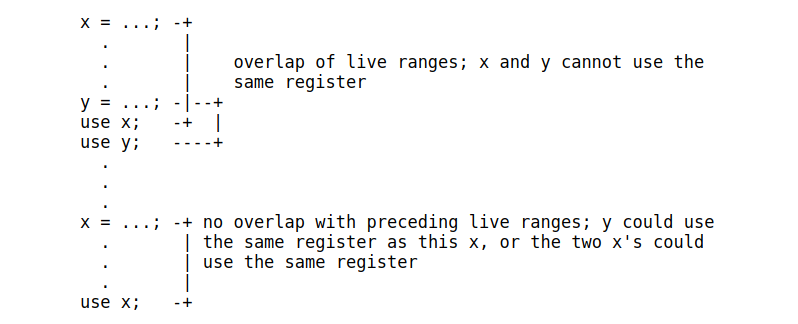
\includegraphics[width=0.6\textwidth]{p164.png}
	\caption{Motivation for graph coloring}
	\label{fig:p164}
\end{figure}


The algorithm for global register allocation via graph coloring consists of 4 steps:
\begin{itemize}
	\item Step 1: Compute live ranges
	\item Step 2: Build the interference graph
	\item Step 3: Color the graph
	\item Step 4: Convert colors to registers
\end{itemize}


\subsubsection{Step 1: compute live ranges}

\begin{itemize}
	\item Build the CFG.
	\item Do reaching defs and live variable analysis.
	      Note: the variables of interest are those that are candidates for registers. Variables that are not candidates might include:
	      \begin{itemize}
		      \item variables that could be aliased:
		            \begin{itemize}
			            \item variables that could be pointed to
			            \item globals (also, could be changed in calls to functions that won't know which register the global is in)
		            \end{itemize}
		      \item array elements (too hard to tell which element is being referred to)
		      \item structs/unions (too big to fit in a register, too hard to deal with individual fields)
		      \item floating-point values (too big to fit in a single register; also, on machines like the Sparc, floating-point registers are not saved across calls)
	      \end{itemize}
	      What's left: locals that are scalar, and not floating point. This might include parameters, though they are sometimes more difficult to handle than "plain" locals.
	\item 	Build initial live ranges:
	      \begin{itemize}
		      \item For each CFG node D that defines variable x, the initial live range for D consists of:

		            \(( <x>, <\{D\} \texttt{  union } \{N | \texttt{x in N.live-before and D in N.reaching-defs-before}\}> ) \)
		            Note: the live range is a pair: the variable defined at D, and the set of nodes in the range.
		      \item Convert initial live ranges to final live ranges (collapse overlapping initial live ranges for the same variable):

		            \begin{figure}[H]
			            \centering
			            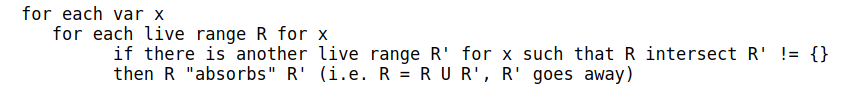
\includegraphics[width=0.6\textwidth]{p165.png}
			            \caption{}
			            \label{fig:p165}
		            \end{figure}


	      \end{itemize}
\end{itemize}


\begin{figure}[H]
	\centering
	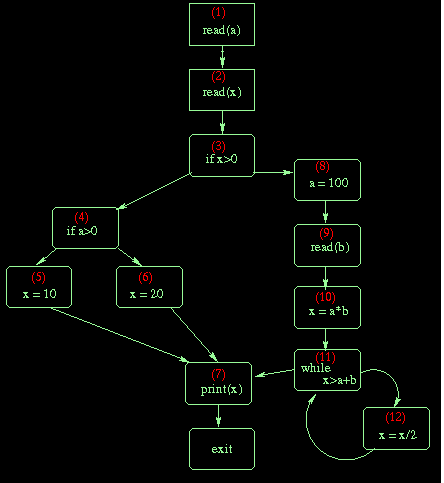
\includegraphics[width=0.6\textwidth]{p166.png}
	\caption{}
	\label{fig:p166}
\end{figure}

\begin{figure}[H]
	\centering
	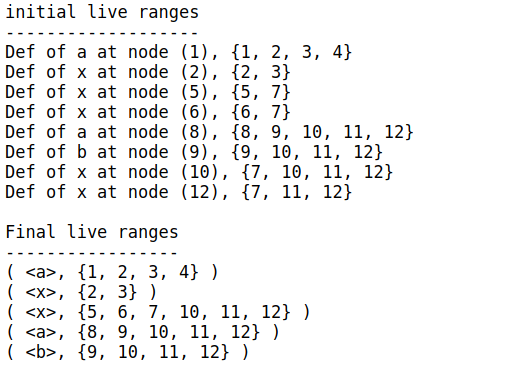
\includegraphics[width=0.6\textwidth]{p168.png}
	\caption{}
	\label{fig:p168}
\end{figure}
\begin{figure}[H]
	\centering
	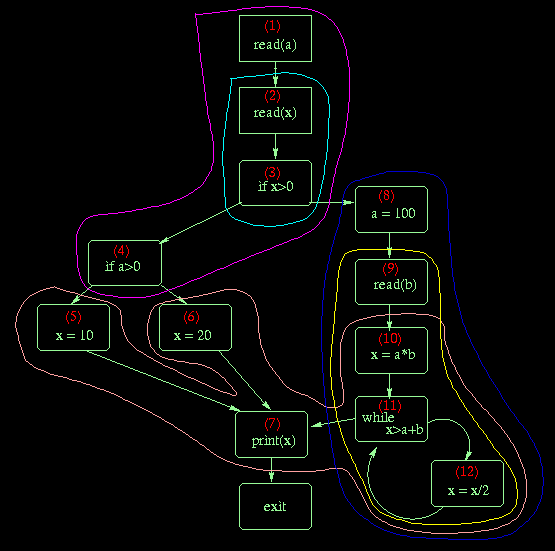
\includegraphics[width=0.6\textwidth]{p167.png}
	\caption{}
	\label{fig:p167}
\end{figure}


\subsubsection{Step 2 - Build the Interference Graph}

\begin{itemize}
	\item 1 node for each live range
	\item 1 undirected edge n-m iff n intersect m != \{\}
\end{itemize}


Here is the graph for the live ranges shown above; the colors used above to encircle the live ranges are used to color the nodes of the interference graph.
\begin{figure}[H]
	\centering
	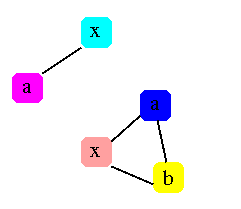
\includegraphics[width=0.6\textwidth]{p169.png}
	\caption{}
	\label{fig:p169}
\end{figure}

% \subsection{Building the Interference Graph}

% Two variables need to be assigned to two different registers if they need to
% hold two different values at some point in the program. This question is
% undecidable in general for programs with loops, so in the context of compilers we reduce this to liveness. A variable is said to be live at a given
% program point if it will used in the remainder of the computation. Again,
% we will not be able to able to accurately predict at compile time whether
% this will be the case, but we can approximate liveness through a particular form of dataflow analysis discussed in the next lecture. In our simple
% straight-line expression language, this is particularly easy. We traverse the
% program backwards, starting at the last line. We note that the return register, \%eax, is live after the last instruction. If a variable is live on one line, it
% is live on the preceding line unless it is assigned to. And a variable that is
% used on the right-hand side of an instruction is live for that instruction.

% As an example, we consider the simple straight-line computation of the
% fifth Fibonacci number, in our pseudo-assembly language. We list with
% each instruction the variables that are live before the line is executed. These
% are called the variables live-in to the instruction.


% \begin{figure}[H]
% 	\centering
% 	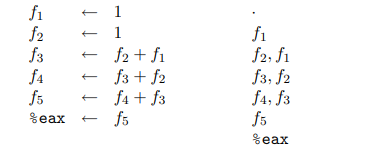
\includegraphics[width=0.4\textwidth]{p153.png}
% 	\caption{}
% 	\label{fig:p153}
% \end{figure}

% The nodes of the interference graph are the variables and registers of the
% program. There is an undirected edge between two nodes if the corresponding variables interfere and should be assigned to different registers.
% There are never edges from a node to itself. We distinguish the two forms
% of instructions.

% \begin{itemize}
% 	\item For an instruction t $\leftarrow$ s1 $\oplus$
% 	      s2 we create an edge between t and any
% 	      different variable $t_i$ live after this line. t and $t_i$ should be assigned to
% 	      different registers, because otherwise the assignment to t could destroy the proper contents of $t_i$
% 	      .
% 	\item For a move instruction t $\leftarrow$ s we create an edge between t and any
% 	      variable $t_i$
% 	      live after this line different from t and s. We omit the potential edge between t and s because if they happen to be assigned to the same register, they still hold the same value after this (now redundant) move. Of course, there may be other occurrences of t and s
% 	      which force them to be assigned to different registers.
% \end{itemize}

% For the above example, we obtain the following interference graph.
% \begin{figure}[H]
% 	\centering
% 	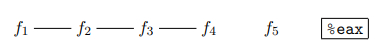
\includegraphics[width=0.4\textwidth]{p154.png}
% 	\caption{}
% 	\label{fig:p154}
% \end{figure}

% Here, the register \%eax is special, because, as a register, it is already predefined and cannot be arbitrarily assigned to another register. Special care
% must be taken with predefined registers during register allocation.




\subsection{ Register Allocation via Graph Coloring}

\begin{figure}[H]
	\centering
	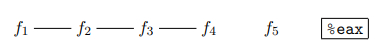
\includegraphics[width=0.4\textwidth]{p154.png}
	\caption{}
	\label{fig:p154}
\end{figure}
Once we have constructed the interference graph, we can pose the register
allocation problem as follows: construct an assignment of K colors (representing K registers) to the nodes of the graph (representing variables)
such that no two connected nodes are of the same color. If no such coloring exists, then we have to save some variables on the stack which is called
spilling.
Unfortunately, the problem whether an arbitrary graph is K-colorable is
NP-complete for K $\geq$ 3. Chaitin\cite{chaitin1982register} has proved that register allocation
is also NP-complete by showing that for any graph G there exists some
program which has G as its interference graph. In other words, one cannot
hope for a theoretically optimal and efficient register allocation algorithm
that works on all machine programs.
Fortunately, in practice the situation is not so dire. One particularly
important intermediate form is static single assignment (SSA). Hack\cite{hack2006register}
observed that for programs in SSA form, the interference graph always has
a specific form called chordal. Coloring for chordal graphs can be accomplished in time $O(|V | + |E|)$ and is quite efficient in practice. Better yet,
Pereira and Palsberg\cite{pereira2005register} noted that as much as 95\% of the programs
occuring in practice have chordal interference graph. Moreover, using the
algorithms designed for chordal graphs behaves well in practice even if
the graph is not quite chordal. Finally, the algorithms needed for coloring
chordal graphs are quite easy to implement compared, for example, to the
complex algorithm in the textbook. You are, of course, free to choose any
algorithm for register allocation you like, but we would suggest one based
on chordal graphs explained in the remainder of this lecture.


\subsection{Chordal Graphs}

An undirected graph is chordal if every cycle with 4 or more nodes has a
chord, that is, an edge not part of the cycle connecting two nodes on the
cycle. Consider the following three examples:
\begin{figure}[H]
	\centering
	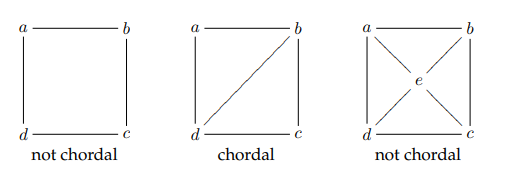
\includegraphics[width=0.4\textwidth]{p155.png}
	\caption{}
	\label{fig:p155}
\end{figure}

chordal chordal not chordal
Only the second one is chordal. In the other two, the cycle abcd does not
have a chord.

On chordal graphs, optimal coloring can be done in two phases, where
optimal means using the minimum number of colors. In the first phase
we determine a particular ordering of the nodes called simplicial elimination
ordering, in the second phase we apply greedy coloring based on this order.


\subsection{Simplicial Elimination Ordering}

plicial Elimination Ordering
A node v in a graph is simplicial if its neighborhood forms a clique, that
is, all neighbors of v are connected to each other. An ordering v1, . . . , vn
of the nodes in a graph is called a simplicial elimination ordering if every
node vi
is simplicial in the subgraph $v_1, \dots , v_i$
. Interestingly, a graph has
a simplicial elimination ordering if and only if it is chordal. We can find
a simplicial elimination ordering using maximum cardinality search, which
can be implemented to run in $O(|V | + |E|)$ time. The algorithm associates
a weight $wt(v)$ with each vertex which is initialized to 0 updated by the
algorithm. We write $N(v)$ for the neighborhood of $v$, that is, the set of all
adjacent nodes.

If the graph is not chordal, the algorithm will still return some ordering
although it will not be simplicial. Such an ordering can still be used in the
coloring phase, but does not guarantee that only the minimal numbers of colors will be used.

\begin{figure}[H]
	\centering
	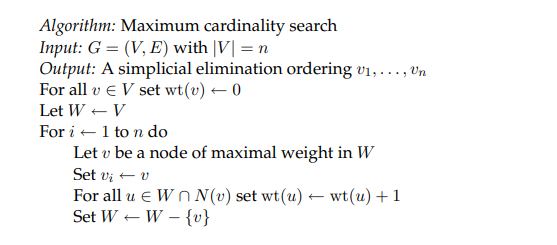
\includegraphics[width=0.4\textwidth]{p156.png}
	\caption{}
	\label{fig:p156}
\end{figure}

In our example \ref{fig:p154},if we pick $f_1$ first, the weight of $f_2$ will become 1 and has
to be picked second, followed by $f_3$ and $f_4$.
Only $f_5$ is left and will come last, ignoring here
\%eax which is already colored. It is easy to see that this is indeed a simplicial
elimination ordering. $f_2, f_4, f_3,\dots$ is not, because the neighborhood of
f3 in the subgraph $f_2, f_4, f_3$ does not form a clique.


\subsection{Greedy Coloring}

Given an ordering, we can apply greedy coloring by simply assigning colors to the
vertices in order, always using the lowest available color. Initially,
no colors are assigned to nodes in $V$ . We write $\Delta(G)$ to the maximum
outdegree of a node in G.


\begin{figure}[H]
	\centering
	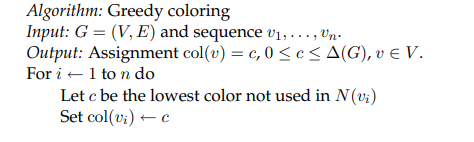
\includegraphics[width=0.4\textwidth]{p157.png}
	\caption{}
	\label{fig:p157}
\end{figure}


The algorithm will always assign at most $\Delta(G)+1$  colors. If the ordering
is a simplicial elimination ordering, the result is furthermore guaranteed to
use the fewest possible colors.

In our example \ref{fig:p154}, we would just alternate color assigments:


\begin{figure}[H]
	\centering
	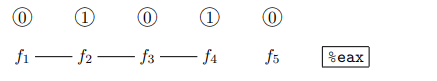
\includegraphics[width=0.4\textwidth]{p158.png}
	\caption{}
	\label{fig:p158}
\end{figure}

Of course, \%eax is represented by one of the colors. Assuming this color is
0 and \%edx is the name of register 1, we obtain the following program:

\begin{figure}[H]
	\centering
	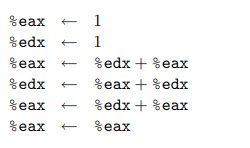
\includegraphics[width=0.4\textwidth]{p159.png}
	\caption{}
	\label{fig:p159}
\end{figure}


It should be apparent that some optimizations are possible. Some are
immediate, such as the redundant move of a register to itself.

\subsection{Register Spilling}


So consider that we have applied the above coloring algorithm and it turns
out that there are more colors needed than registers available. In that case
we need to save some temporary values. In our runtime architecture, the
stack is the obvious place. One convenient way to achieve this is to simply
assign stack slots instead of registers to some of the colors. The choice of
which colors to spill can have a drastic impact on the running time. Pereira
and Palsberg suggest two heuristics: (i) spill the least-used color, and (ii)
spill the highest color assigned by the greedy algorithm. For programs with
loops and nested loops, it may also be significant where in the programs the
variables or certain colors are used: keeping variables used frequently in
inner loops may be crucial for certain programs.
Once we have assigned stack slots to colors, it is easy to rewrite the code
using temps that are spilled if we reserve a register in advance for moves
to and from the stack when necessary. For example, if \%r11 on the x86-64
is reserved to implement save and restore when necessary, then \(t \leftarrow t + s \)
where t is assigned to stack offset 8 and s to \%eax can be rewritten to

\begin{figure}[H]
	\centering
	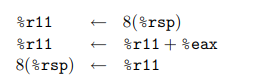
\includegraphics[width=0.4\textwidth]{p160.png}
	\caption{}
	\label{fig:p160}
\end{figure}


Sometimes, this is unnecessary because some operations can be carried
out directly with memory references. So the assembly code for the above
could be shorter

\begin{figure}[H]
	\centering
	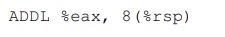
\includegraphics[width=0.4\textwidth]{p161.png}
	\caption{}
	\label{fig:p161}
\end{figure}

although it is not clear whether and how much more efficient this might be
than a 3-instruction sequence

\begin{figure}[H]
	\centering
	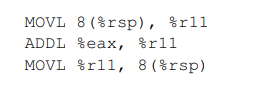
\includegraphics[width=0.4\textwidth]{p162.png}
	\caption{}
	\label{fig:p162}
\end{figure}

We recommend generating the simplest uniform instruction sequences for
spill code.

\subsection{Register Coalescing}


After register allocation, a common further optimization is used to eliminate register-to-register moves called register coalescing. Algorithms for
register coalescing are usually tightly integrated with register allocation. In
contrast, Pereira and Palsberg describe a relatively straightforward method
that is performed entirely after graph coloring called greedy coalescing.


The algorithm considers each move between variables $t \leftarrow s$ occurring
in the program in turn. If t and s they are the same color, the move can be
eliminated without further action. If there is an edge between them, that
is, they interfere, they cannot be coalesced. Otherwise, if there is a color c
which is not used in the neighborhoods of t and s, $N(t) U N(s)$, and which is
smaller than the number of available registers, then the variables t and s are
coalesced into a single new variable u with color c. We create edges from u
to any vertex in $N(t) U N(s)$ and remove t and s from the graph. Because
of the tested condition, the resulting graph is still K-colored, where K is
the number of available registers. Of course, we also need to eventually
rewrite the program appropriately to maintain a correspondence with the graph.

\subsection{ Precolored Nodes}
Some instructions on the x86-64, such as IDIV, require their arguments to
be passed in specific registers and return their results also in specific registers. There are also call and ret instructions that use specific registers
and must respect caller-save and callee-save register conventions. We will
return to the issue of calling conventions later in the course. When generating code for a straight-line program as in the first lab, some care must be
taken to save and restore callee-save registers in case they are needed.
First, for code generation, the live range of the fixed registers should be
limited to avoid possible correctness issues and simplify register allocation.
Second, for register allocation, we can construct an elimination ordering as if all precolored nodes were listed first. This amounts to the initial weights of the ordinary vertices being set to the number of neighbors
that are precolored before the maximum cardinality search algorithm starts.
The resulting list may or may not be a simplicial elimination ordering, but
we can nevertheless proceed with greedy coloring as before.



\subsection{Example : }

The live range for a variable is the set of program
points at which that variable is live.

The live interval for a variable is the smallest
subrange of the IR code containing all a variable's
live ranges. Less precise than live ranges, but simpler to work with.

Linear Scan use live interval, graph coloring uses live range.


\subsection{Problem Set}

\begin{problem}
Register Allocation.

\begin{center}
	\begin{tikzpicture}
		\node[bb] (entry) {\entry};
		\node[bb, below=1em of entry, label={left:B1}] (a1)  {$\begin{aligned}A&=9;\\D&=0;\\E&=5;\end{aligned}$};
		\node[bb, below left=1em and 2em of a1, label={left:B2}] (b1) {$C=A-2;$};
		\node[bb, below right=1em and 2em of a1, label={right:B3}] (c1) {$B=A+5;$};
		\node[bb, below right=2em and 2em of b1, label={above:B4}] (a2) {$\begin{aligned}D&=E-2;\\E&=12;\end{aligned}$};
		\node[bb, below=2em of c1, label={right:B5}] (c2) {$C=B+2;$};
		\node[bb, below=2em of c2, label={right:B6}] (c3) {$E=E-C;$};
		\node[bb, below=2em of b1, label={above left:B7}] (b2) {$B=D+7;$};
		\node[bb, below=2em of b2, label={above left:B8}] (b3) {$D=B-2;$};
		\node[bb, below left=-1em and 2em of b2, label={left:B9}] (e1) {$\begin{aligned}C&=B+1;\\D&=C+1;\\B&=D+6;\end{aligned}$};
		\node[bb, below=4em of a2, label={left:B10}] (a3) {$E=D+E;$};
		\node[bb, below=1em of a3] (exit) {\exit};


		\draw[->] (entry) -- (a1);
		\draw[->] (a1) -- (b1);
		\draw[->] (b1) -- (b2);
		\draw[->] (b2) -- (b3);
		\draw[->] (b3) to [out=0,in=0] (b2);
		\draw[->] (b2) -- (e1);
		\draw[->] (e1) -- (b3);
		\draw[->] (a1) -- (c1);
		\draw[->] (c1) -- (c2);
		\draw[->] (c2) -- (c3);
		\draw[->] (c3) -- (a3);
		\draw[->] (c1) -- (a2);
		\draw[->] (b1) -- (a2);
		\draw[->] (a2) -- (c3);
		\draw[->] (b3) -- (a3);
		\draw[->] (c3) -- (a3);
		\draw[->] (a3) -- (exit);
	\end{tikzpicture}
\end{center}

\item Perform register allocation for the above control flow graph.
Specifically, show the results of each of the following steps:
\begin{enumerate}
	\item Show the merged live ranges for the following program by updating the graph with unique variable notations, e.g., replace definitions and usages of $B$ with $B_1$, $B_2$, etc. Note: if different definitions form a merged live range, use the same variable notation (you may convince yourself that this avoids ambiguity when a used variable may come from different definitions).
	      We provide you with an example. For the following simple program:
	      \begin{center}
		      \begin{tikzpicture}
			      \node[bb] (entry) {\entry};
			      \node[bb, below=1em of entry, label={left:B1}] (a1)  {$\begin{aligned}A=0;\\C=0;\end{aligned}$};
			      \node[bb, below left=0.5em and 2em of a1, label={left:B2}] (a2)  {$\begin{aligned}A=1;\\B=1;\end{aligned}$};
			      \node[bb, below right=1em and 2em of a1, label={left:B3}] (a3)  {$A=2;$};
			      \node[bb, below=4em of a1, label={left:B4}] (a4)  {$B=A + C;$};
			      \node[bb, below=1em of a4] (exit) {\exit};

			      \draw[->] (entry) -- (a1);
			      \draw[->] (a1) -- (a2);
			      \draw[->] (a1) -- (a3);
			      \draw[->] (a2) -- (a4);
			      \draw[->] (a3) -- (a4);
			      \draw[->] (a4) -- (exit);
		      \end{tikzpicture}
	      \end{center}
	      The resulting updated graph is:
	      \begin{center}
		      \begin{tikzpicture}
			      \node[bb] (entry) {\entry};
			      \node[bb, below=1em of entry, label={left:B1}] (a1)  {$\begin{aligned}A_1&=0;\\C_1&=0;\end{aligned}$};
			      \node[bb, below left=0.5em and 2em of a1, label={left:B2}] (a2)  {$\begin{aligned}A_2&=1;\\B_1&=1;\end{aligned}$};
			      \node[bb, below right=1em and 2em of a1, label={left:B3}] (a3)  {$A_2=2;$};
			      \node[bb, below=4em of a1, label={left:B4}] (a4)  {$B_2=A_2 + C_1;$};
			      \node[bb, below=1em of a4] (exit) {\exit};

			      \draw[->] (entry) -- (a1);
			      \draw[->] (a1) -- (a2);
			      \draw[->] (a1) -- (a3);
			      \draw[->] (a2) -- (a4);
			      \draw[->] (a3) -- (a4);
			      \draw[->] (a4) -- (exit);
		      \end{tikzpicture}
	      \end{center}
	      Taking the definitions of $A$ in B2 and B3 as example, $A$ is live at the beginning of B4, and both definitions reach that point, therefore they can be merged. \textbf{Note:} you do not need to consider any optimization such as PRE or constant propagation.
	\item Draw the register interference graph with edges between nodes that represent merged live ranges. Using the same example program, the register inference graph should look like:
	      \begin{center}
		      \begin{tikzpicture}[lr/.style={draw, circle, radius=6em, align=center, font=\mathstrut}]
			      \node[lr] (n1) {$A_1$};
			      \node[lr, below=1em of n1] (n2) {$A_2$};
			      \node[lr, right=1em of n1] (n3) {$B_1$};
			      \node[lr, below=1em of n3] (n4) {$B_2$};
			      \node[lr, right=1em of n3] (n5) {$C_1$};
			      \draw (n2) -- (n5);
		      \end{tikzpicture}
	      \end{center}
	\item Apply the coloring algorithm for a machine with 3 registers to the interference graph from the previous part. Show a possible resulting ``stack'' of registers and show which ones, if any, are marked as spilled.
	\item Assign the merged live ranges (i.e., $A_1, B_1, ...$) to registers. You may assume the three registers are labeled as $R_1, R_2, R_3$.
\end{enumerate}

\newpage
\end{problem}

\begin{problem}
Register Allocation and Live Ranges.

\begin{problempart}
	Let $n$ be the largest number of overlapping live ranges seen in a program.
	\begin{enumerate}
		\item Is it possible to assign all variables to registers on a machine with $n - 1$ registers, without spilling? Explain your answer.
		\item Is it always possible to find a register allocation on a machine with $n$ registers, without spilling? Explain your answer.
	\end{enumerate}
\end{problempart}
\begin{problempart}
	Observe the control-flow graph below and answer the following questions.
	\begin{enumerate}
		\item What is the largest number of overlapping live ranges seen at any program point?
		\item What is the minimum number of registers you need in order to successfully assign all variables without spilling?
		\item Now, imagine that, as part of register allocation, you can insert \texttt{MOVE x y} operations that copy a value from register \texttt{x} to another register \texttt{y}. Can you allocate all of the variables with fewer registers than before? If so, how many would it require?
	\end{enumerate}
\end{problempart}

\begin{center}
	\begin{tikzpicture}[placeholder/.append style={text width=5em}]
		\node[bb] (entry) {\entry};
		\node[bb, below=1em of entry] (pre) {$\begin{aligned} B &= \ldots \\ C &= \ldots \end{aligned}$};
		\node[bb, below=1em of pre] (loop) {$\begin{gathered}
					\mathrm{print}(C) \\
					A = \ldots \\
					\mathrm{print}(B) \\
					C = \ldots \\
					\mathrm{print}(A) \\
					B = \ldots
				\end{gathered}$};
		\node[bb, below=1em of loop] (exit) {\exit};

		\draw[->] (entry) -- (pre);
		\draw[->] (pre) -- (loop);
		\draw[->] (loop) .. controls +(-130:4) and +(+130:4) .. (loop);
		\draw[->] (loop) -- (exit);
	\end{tikzpicture}
\end{center}

\newpage
\end{problem}


\subsection{Summary}

linear scan register allocation Advantages:

\begin{itemize}
	\item Very efficient (after computing live intervals, runs in linear
	      time)
	\item Produces good code in many instances.
	\item Allocation step works in one pass; can generate code during
	      iteration.
	\item Often used in JIT compilers like Java HotSpot.
\end{itemize}
Disadvantages:
\begin{itemize}
	\item Imprecise due to use of live intervals rather than live ranges.
	\item Other techniques known to be superior in many cases.
\end{itemize}